\documentclass[1p]{elsarticle_modified}
%\bibliographystyle{elsarticle-num}

%\usepackage[colorlinks]{hyperref}
%\usepackage{abbrmath_seonhwa} %\Abb, \Ascr, \Acal ,\Abf, \Afrak
\usepackage{amsfonts}
\usepackage{amssymb}
\usepackage{amsmath}
\usepackage{amsthm}
\usepackage{scalefnt}
\usepackage{amsbsy}
\usepackage{kotex}
\usepackage{caption}
\usepackage{subfig}
\usepackage{color}
\usepackage{graphicx}
\usepackage{xcolor} %% white, black, red, green, blue, cyan, magenta, yellow
\usepackage{float}
\usepackage{setspace}
\usepackage{hyperref}

\usepackage{tikz}
\usetikzlibrary{arrows}

\usepackage{multirow}
\usepackage{array} % fixed length table
\usepackage{hhline}

%%%%%%%%%%%%%%%%%%%%%
\makeatletter
\renewcommand*\env@matrix[1][\arraystretch]{%
	\edef\arraystretch{#1}%
	\hskip -\arraycolsep
	\let\@ifnextchar\new@ifnextchar
	\array{*\c@MaxMatrixCols c}}
\makeatother %https://tex.stackexchange.com/questions/14071/how-can-i-increase-the-line-spacing-in-a-matrix
%%%%%%%%%%%%%%%

\usepackage[normalem]{ulem}

\newcommand{\msout}[1]{\ifmmode\text{\sout{\ensuremath{#1}}}\else\sout{#1}\fi}
%SOURCE: \msout is \stkout macro in https://tex.stackexchange.com/questions/20609/strikeout-in-math-mode

\newcommand{\cancel}[1]{
	\ifmmode
	{\color{red}\msout{#1}}
	\else
	{\color{red}\sout{#1}}
	\fi
}

\newcommand{\add}[1]{
	{\color{blue}\uwave{#1}}
}

\newcommand{\replace}[2]{
	\ifmmode
	{\color{red}\msout{#1}}{\color{blue}\uwave{#2}}
	\else
	{\color{red}\sout{#1}}{\color{blue}\uwave{#2}}
	\fi
}

\newcommand{\Sol}{\mathcal{S}} %segment
\newcommand{\D}{D} %diagram
\newcommand{\A}{\mathcal{A}} %arc


%%%%%%%%%%%%%%%%%%%%%%%%%%%%%5 test

\def\sl{\operatorname{\textup{SL}}(2,\Cbb)}
\def\psl{\operatorname{\textup{PSL}}(2,\Cbb)}
\def\quan{\mkern 1mu \triangleright \mkern 1mu}

\theoremstyle{definition}
\newtheorem{thm}{Theorem}[section]
\newtheorem{prop}[thm]{Proposition}
\newtheorem{lem}[thm]{Lemma}
\newtheorem{ques}[thm]{Question}
\newtheorem{cor}[thm]{Corollary}
\newtheorem{defn}[thm]{Definition}
\newtheorem{exam}[thm]{Example}
\newtheorem{rmk}[thm]{Remark}
\newtheorem{alg}[thm]{Algorithm}

\newcommand{\I}{\sqrt{-1}}
\begin{document}

%\begin{frontmatter}
%
%\title{Boundary parabolic representations of knots up to 8 crossings}
%
%%% Group authors per affiliation:
%\author{Yunhi Cho} 
%\address{Department of Mathematics, University of Seoul, Seoul, Korea}
%\ead{yhcho@uos.ac.kr}
%
%
%\author{Seonhwa Kim} %\fnref{s_kim}}
%\address{Center for Geometry and Physics, Institute for Basic Science, Pohang, 37673, Korea}
%\ead{ryeona17@ibs.re.kr}
%
%\author{Hyuk Kim}
%\address{Department of Mathematical Sciences, Seoul National University, Seoul 08826, Korea}
%\ead{hyukkim@snu.ac.kr}
%
%\author{Seokbeom Yoon}
%\address{Department of Mathematical Sciences, Seoul National University, Seoul, 08826,  Korea}
%\ead{sbyoon15@snu.ac.kr}
%
%\begin{abstract}
%We find all boundary parabolic representation of knots up to 8 crossings.
%
%\end{abstract}
%\begin{keyword}
%    \MSC[2010] 57M25 
%\end{keyword}
%
%\end{frontmatter}

%\linenumbers
%\tableofcontents
%
\newcommand\colored[1]{\textcolor{white}{\rule[-0.35ex]{0.8em}{1.4ex}}\kern-0.8em\color{red} #1}%
%\newcommand\colored[1]{\textcolor{white}{ #1}\kern-2.17ex	\textcolor{white}{ #1}\kern-1.81ex	\textcolor{white}{ #1}\kern-2.15ex\color{red}#1	}

{\Large $\underline{11a_{134}~(K11a_{134})}$}

\setlength{\tabcolsep}{10pt}
\renewcommand{\arraystretch}{1.6}
\vspace{1cm}\begin{tabular}{m{100pt}>{\centering\arraybackslash}m{274pt}}
\multirow{5}{120pt}{
	\centering
	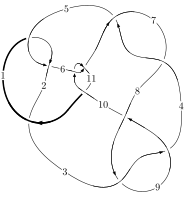
\includegraphics[width=112pt]{../../../GIT/diagram.site/Diagrams/png/383_11a_134.png}\\
\ \ \ A knot diagram\footnotemark}&
\allowdisplaybreaks
\textbf{Linearized knot diagam} \\
\cline{2-2}
 &
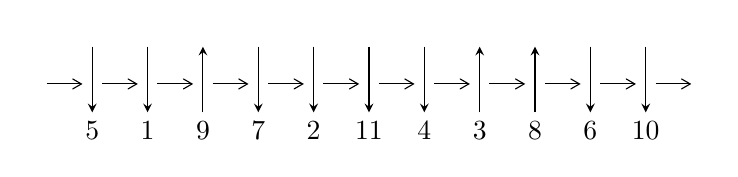
\begin{tikzpicture}[x=20pt, y=17pt]
	% nodes
	\node (C0) at (0, 0) {};
	\node (C1) at (1, 0) {};
	\node (C1U) at (1, +1) {};
	\node (C1D) at (1, -1) {5};

	\node (C2) at (2, 0) {};
	\node (C2U) at (2, +1) {};
	\node (C2D) at (2, -1) {1};

	\node (C3) at (3, 0) {};
	\node (C3U) at (3, +1) {};
	\node (C3D) at (3, -1) {9};

	\node (C4) at (4, 0) {};
	\node (C4U) at (4, +1) {};
	\node (C4D) at (4, -1) {7};

	\node (C5) at (5, 0) {};
	\node (C5U) at (5, +1) {};
	\node (C5D) at (5, -1) {2};

	\node (C6) at (6, 0) {};
	\node (C6U) at (6, +1) {};
	\node (C6D) at (6, -1) {11};

	\node (C7) at (7, 0) {};
	\node (C7U) at (7, +1) {};
	\node (C7D) at (7, -1) {4};

	\node (C8) at (8, 0) {};
	\node (C8U) at (8, +1) {};
	\node (C8D) at (8, -1) {3};

	\node (C9) at (9, 0) {};
	\node (C9U) at (9, +1) {};
	\node (C9D) at (9, -1) {8};

	\node (C10) at (10, 0) {};
	\node (C10U) at (10, +1) {};
	\node (C10D) at (10, -1) {6};

	\node (C11) at (11, 0) {};
	\node (C11U) at (11, +1) {};
	\node (C11D) at (11, -1) {10};
	\node (C12) at (12, 0) {};

	% arrows
	\draw[->,>={angle 60}]
	(C0) edge (C1) (C1) edge (C2) (C2) edge (C3) (C3) edge (C4) (C4) edge (C5) (C5) edge (C6) (C6) edge (C7) (C7) edge (C8) (C8) edge (C9) (C9) edge (C10) (C10) edge (C11) (C11) edge (C12) ;	\draw[->,>=stealth]
	(C1U) edge (C1D) (C2U) edge (C2D) (C3D) edge (C3U) (C4U) edge (C4D) (C5U) edge (C5D) (C6U) edge (C6D) (C7U) edge (C7D) (C8D) edge (C8U) (C9D) edge (C9U) (C10U) edge (C10D) (C11U) edge (C11D) ;
	\end{tikzpicture} \\
\hhline{~~} \\& 
\textbf{Solving Sequence} \\ \cline{2-2} 
 &
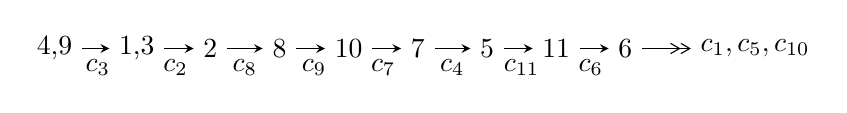
\begin{tikzpicture}[x=25pt, y=7pt]
	% node
	\node (A0) at (-1/8, 0) {4,9};
	\node (A1) at (17/16, 0) {1,3};
	\node (A2) at (17/8, 0) {2};
	\node (A3) at (25/8, 0) {8};
	\node (A4) at (33/8, 0) {10};
	\node (A5) at (41/8, 0) {7};
	\node (A6) at (49/8, 0) {5};
	\node (A7) at (57/8, 0) {11};
	\node (A8) at (65/8, 0) {6};
	\node (C1) at (1/2, -1) {$c_{3}$};
	\node (C2) at (13/8, -1) {$c_{2}$};
	\node (C3) at (21/8, -1) {$c_{8}$};
	\node (C4) at (29/8, -1) {$c_{9}$};
	\node (C5) at (37/8, -1) {$c_{7}$};
	\node (C6) at (45/8, -1) {$c_{4}$};
	\node (C7) at (53/8, -1) {$c_{11}$};
	\node (C8) at (61/8, -1) {$c_{6}$};
	\node (A9) at (10, 0) {$c_{1},c_{5},c_{10}$};

	% edge
	\draw[->,>=stealth]	
	(A0) edge (A1) (A1) edge (A2) (A2) edge (A3) (A3) edge (A4) (A4) edge (A5) (A5) edge (A6) (A6) edge (A7) (A7) edge (A8) ;
	\draw[->>,>={angle 60}]	
	(A8) edge (A9);
\end{tikzpicture} \\ 

\end{tabular} \\

\footnotetext{
The image of knot diagram is generated by the software ``\textbf{Draw programme}" developed by Andrew Bartholomew(\url{http://www.layer8.co.uk/maths/draw/index.htm\#Running-draw}), where we modified some parts for our purpose(\url{https://github.com/CATsTAILs/LinksPainter}).
}\phantom \\ \newline 
\centering \textbf{Ideals for irreducible components\footnotemark of $X_{\text{par}}$} 
 
\begin{align*}
I^u_{1}&=\langle 
-2 u^{27}-5 u^{26}+\cdots+b-5,\;-5 u^{27}-11 u^{26}+\cdots+2 a-10,\;u^{28}+3 u^{27}+\cdots+6 u+2\rangle \\
I^u_{2}&=\langle 
2 u^{19} a+292 u^{19}+\cdots-19 a+450,\;-2 u^{19} a+u^{19}+\cdots-4 a+1,\;u^{20}- u^{19}+\cdots+2 u-1\rangle \\
I^u_{3}&=\langle 
u^3+b- u-1,\;u^3+2 u^2+2 a-4,\;u^4-2 u^2+2\rangle \\
\\
I^v_{1}&=\langle 
a,\;b+1,\;v+1\rangle \\
\end{align*}
\raggedright * 4 irreducible components of $\dim_{\mathbb{C}}=0$, with total 73 representations.\\
\footnotetext{All coefficients of polynomials are rational numbers. But the coefficients are sometimes approximated in decimal forms when there is not enough margin.}
\newpage
\renewcommand{\arraystretch}{1}
\centering \section*{I. $I^u_{1}= \langle -2 u^{27}-5 u^{26}+\cdots+b-5,\;-5 u^{27}-11 u^{26}+\cdots+2 a-10,\;u^{28}+3 u^{27}+\cdots+6 u+2 \rangle$}
\flushleft \textbf{(i) Arc colorings}\\
\begin{tabular}{m{7pt} m{180pt} m{7pt} m{180pt} }
\flushright $a_{4}=$&$\begin{pmatrix}1\\0\end{pmatrix}$ \\
\flushright $a_{9}=$&$\begin{pmatrix}0\\u\end{pmatrix}$ \\
\flushright $a_{1}=$&$\begin{pmatrix}\frac{5}{2} u^{27}+\frac{11}{2} u^{26}+\cdots+11 u+5\\2 u^{27}+5 u^{26}+\cdots+11 u+5\end{pmatrix}$ \\
\flushright $a_{3}=$&$\begin{pmatrix}1\\u^2\end{pmatrix}$ \\
\flushright $a_{2}=$&$\begin{pmatrix}-\frac{3}{2} u^{27}-\frac{7}{2} u^{26}+\cdots-7 u-2\\- u^{27}-3 u^{26}+\cdots-7 u-3\end{pmatrix}$ \\
\flushright $a_{8}=$&$\begin{pmatrix}- u\\- u^3+u\end{pmatrix}$ \\
\flushright $a_{10}=$&$\begin{pmatrix}u^3\\u^5- u^3+u\end{pmatrix}$ \\
\flushright $a_{7}=$&$\begin{pmatrix}- u^3\\- u^3+u\end{pmatrix}$ \\
\flushright $a_{5}=$&$\begin{pmatrix}u^6- u^4+1\\u^6-2 u^4+u^2\end{pmatrix}$ \\
\flushright $a_{11}=$&$\begin{pmatrix}\frac{3}{2} u^{27}+\frac{7}{2} u^{26}+\cdots+7 u+3\\u^{27}+3 u^{26}+\cdots+6 u+3\end{pmatrix}$ \\
\flushright $a_{6}=$&$\begin{pmatrix}\frac{3}{2} u^{27}+\frac{7}{2} u^{26}+\cdots+7 u+3\\- u^{27}-2 u^{26}+\cdots-3 u-1\end{pmatrix}$\\ \flushright $a_{6}=$&$\begin{pmatrix}\frac{3}{2} u^{27}+\frac{7}{2} u^{26}+\cdots+7 u+3\\- u^{27}-2 u^{26}+\cdots-3 u-1\end{pmatrix}$\\&\end{tabular}
\flushleft \textbf{(ii) Obstruction class $= -1$}\\~\\
\flushleft \textbf{(iii) Cusp Shapes $= 16 u^{27}+34 u^{26}-80 u^{25}-254 u^{24}+90 u^{23}+816 u^{22}+388 u^{21}-1304 u^{20}-1582 u^{19}+636 u^{18}+2460 u^{17}+1314 u^{16}-1448 u^{15}-2534 u^{14}-826 u^{13}+1418 u^{12}+1758 u^{11}+426 u^{10}-722 u^9-752 u^8-194 u^7+132 u^6+96 u^5-4 u^4+10 u^3+68 u^2+70 u+24$}\\~\\
\newpage\renewcommand{\arraystretch}{1}
\flushleft \textbf{(iv) u-Polynomials at the component}\newline \\
\begin{tabular}{m{50pt}|m{274pt}}
Crossings & \hspace{64pt}u-Polynomials at each crossing \\
\hline $$\begin{aligned}c_{1},c_{5},c_{6}\\c_{10}\end{aligned}$$&$\begin{aligned}
&u^{28}+u^{27}+\cdots-5 u^2+1
\end{aligned}$\\
\hline $$\begin{aligned}c_{2},c_{11}\end{aligned}$$&$\begin{aligned}
&u^{28}+11 u^{27}+\cdots+10 u+1
\end{aligned}$\\
\hline $$\begin{aligned}c_{3},c_{8}\end{aligned}$$&$\begin{aligned}
&u^{28}-3 u^{27}+\cdots-6 u+2
\end{aligned}$\\
\hline $$\begin{aligned}c_{4},c_{7}\end{aligned}$$&$\begin{aligned}
&u^{28}-9 u^{27}+\cdots-118 u+14
\end{aligned}$\\
\hline $$\begin{aligned}c_{9}\end{aligned}$$&$\begin{aligned}
&u^{28}-15 u^{27}+\cdots-4 u+4
\end{aligned}$\\
\hline
\end{tabular}\\~\\
\newpage\renewcommand{\arraystretch}{1}
\flushleft \textbf{(v) Riley Polynomials at the component}\newline \\
\begin{tabular}{m{50pt}|m{274pt}}
Crossings & \hspace{64pt}Riley Polynomials at each crossing \\
\hline $$\begin{aligned}c_{1},c_{5},c_{6}\\c_{10}\end{aligned}$$&$\begin{aligned}
&y^{28}-11 y^{27}+\cdots-10 y+1
\end{aligned}$\\
\hline $$\begin{aligned}c_{2},c_{11}\end{aligned}$$&$\begin{aligned}
&y^{28}+21 y^{27}+\cdots-6 y+1
\end{aligned}$\\
\hline $$\begin{aligned}c_{3},c_{8}\end{aligned}$$&$\begin{aligned}
&y^{28}-15 y^{27}+\cdots-4 y+4
\end{aligned}$\\
\hline $$\begin{aligned}c_{4},c_{7}\end{aligned}$$&$\begin{aligned}
&y^{28}+21 y^{27}+\cdots+2092 y+196
\end{aligned}$\\
\hline $$\begin{aligned}c_{9}\end{aligned}$$&$\begin{aligned}
&y^{28}-3 y^{27}+\cdots+112 y+16
\end{aligned}$\\
\hline
\end{tabular}\\~\\
\newpage\flushleft \textbf{(vi) Complex Volumes and Cusp Shapes}
$$\begin{array}{c|c|c}  
\text{Solutions to }I^u_{1}& \I (\text{vol} + \sqrt{-1}CS) & \text{Cusp shape}\\
 \hline 
\begin{aligned}
u &= -0.921184 + 0.300728 I \\
a &= \phantom{-}0.870295 - 0.372461 I \\
b &= \phantom{-}0.659106 - 0.511462 I\end{aligned}
 & \phantom{-}1.56197 - 1.13269 I & \phantom{-}1.72628 + 0.97911 I \\ \hline\begin{aligned}
u &= -0.921184 - 0.300728 I \\
a &= \phantom{-}0.870295 + 0.372461 I \\
b &= \phantom{-}0.659106 + 0.511462 I\end{aligned}
 & \phantom{-}1.56197 + 1.13269 I & \phantom{-}1.72628 - 0.97911 I \\ \hline\begin{aligned}
u &= -0.879043 + 0.588894 I \\
a &= -1.46570 + 0.82867 I \\
b &= -0.651267 + 0.638133 I\end{aligned}
 & -2.48501 - 9.60327 I & -7.71691 + 9.77284 I \\ \hline\begin{aligned}
u &= -0.879043 - 0.588894 I \\
a &= -1.46570 - 0.82867 I \\
b &= -0.651267 - 0.638133 I\end{aligned}
 & -2.48501 + 9.60327 I & -7.71691 - 9.77284 I \\ \hline\begin{aligned}
u &= -0.644981 + 0.626187 I \\
a &= \phantom{-}0.089635 + 0.895732 I \\
b &= -0.092830 + 1.067970 I\end{aligned}
 & -3.15613 + 4.86238 I & -9.07167 - 4.07725 I \\ \hline\begin{aligned}
u &= -0.644981 - 0.626187 I \\
a &= \phantom{-}0.089635 - 0.895732 I \\
b &= -0.092830 - 1.067970 I\end{aligned}
 & -3.15613 - 4.86238 I & -9.07167 + 4.07725 I \\ \hline\begin{aligned}
u &= \phantom{-}1.099790 + 0.120657 I \\
a &= \phantom{-}0.57327 - 1.71129 I \\
b &= \phantom{-}0.677548 - 0.714007 I\end{aligned}
 & \phantom{-}2.55286 + 5.06128 I & -0.17487 - 6.03485 I \\ \hline\begin{aligned}
u &= \phantom{-}1.099790 - 0.120657 I \\
a &= \phantom{-}0.57327 + 1.71129 I \\
b &= \phantom{-}0.677548 + 0.714007 I\end{aligned}
 & \phantom{-}2.55286 - 5.06128 I & -0.17487 + 6.03485 I \\ \hline\begin{aligned}
u &= -0.158971 + 0.833066 I \\
a &= -0.681108 - 0.773177 I \\
b &= -0.64725 + 2.19051 I\end{aligned}
 & \phantom{-}1.27438 + 10.50480 I & -6.28570 - 6.88896 I \\ \hline\begin{aligned}
u &= -0.158971 - 0.833066 I \\
a &= -0.681108 + 0.773177 I \\
b &= -0.64725 - 2.19051 I\end{aligned}
 & \phantom{-}1.27438 - 10.50480 I & -6.28570 + 6.88896 I\\
 \hline 
 \end{array}$$\newpage$$\begin{array}{c|c|c}  
\text{Solutions to }I^u_{1}& \I (\text{vol} + \sqrt{-1}CS) & \text{Cusp shape}\\
 \hline 
\begin{aligned}
u &= \phantom{-}1.050730 + 0.482260 I \\
a &= \phantom{-}0.437094 - 0.465500 I \\
b &= \phantom{-}0.469489 + 0.315915 I\end{aligned}
 & \phantom{-}0.63188 + 4.55606 I & -2.14668 - 8.40653 I \\ \hline\begin{aligned}
u &= \phantom{-}1.050730 - 0.482260 I \\
a &= \phantom{-}0.437094 + 0.465500 I \\
b &= \phantom{-}0.469489 - 0.315915 I\end{aligned}
 & \phantom{-}0.63188 - 4.55606 I & -2.14668 + 8.40653 I \\ \hline\begin{aligned}
u &= -0.045051 + 0.816095 I \\
a &= \phantom{-}0.601069 + 0.545123 I \\
b &= -0.048727 - 1.403620 I\end{aligned}
 & \phantom{-}4.78070 - 0.80383 I & -1.62038 + 2.30991 I \\ \hline\begin{aligned}
u &= -0.045051 - 0.816095 I \\
a &= \phantom{-}0.601069 - 0.545123 I \\
b &= -0.048727 + 1.403620 I\end{aligned}
 & \phantom{-}4.78070 + 0.80383 I & -1.62038 - 2.30991 I \\ \hline\begin{aligned}
u &= -1.083610 + 0.529736 I \\
a &= \phantom{-}1.44141 + 0.49547 I \\
b &= \phantom{-}1.244770 - 0.462759 I\end{aligned}
 & \phantom{-}0.11867 - 1.62470 I & -4.25246 - 1.50082 I \\ \hline\begin{aligned}
u &= -1.083610 - 0.529736 I \\
a &= \phantom{-}1.44141 - 0.49547 I \\
b &= \phantom{-}1.244770 + 0.462759 I\end{aligned}
 & \phantom{-}0.11867 + 1.62470 I & -4.25246 + 1.50082 I \\ \hline\begin{aligned}
u &= -0.362452 + 0.684626 I \\
a &= \phantom{-}0.114239 - 0.531482 I \\
b &= -0.940476 - 0.787619 I\end{aligned}
 & -1.97520 - 3.04297 I & -7.88705 + 5.30670 I \\ \hline\begin{aligned}
u &= -0.362452 - 0.684626 I \\
a &= \phantom{-}0.114239 + 0.531482 I \\
b &= -0.940476 + 0.787619 I\end{aligned}
 & -1.97520 + 3.04297 I & -7.88705 - 5.30670 I \\ \hline\begin{aligned}
u &= \phantom{-}1.228580 + 0.361628 I \\
a &= \phantom{-}1.30002 + 1.89665 I \\
b &= -0.70865 + 2.23120 I\end{aligned}
 & \phantom{-}5.53046 - 6.50130 I & -1.52112 + 3.99395 I \\ \hline\begin{aligned}
u &= \phantom{-}1.228580 - 0.361628 I \\
a &= \phantom{-}1.30002 - 1.89665 I \\
b &= -0.70865 - 2.23120 I\end{aligned}
 & \phantom{-}5.53046 + 6.50130 I & -1.52112 - 3.99395 I\\
 \hline 
 \end{array}$$\newpage$$\begin{array}{c|c|c}  
\text{Solutions to }I^u_{1}& \I (\text{vol} + \sqrt{-1}CS) & \text{Cusp shape}\\
 \hline 
\begin{aligned}
u &= \phantom{-}1.223330 + 0.431243 I \\
a &= -0.56938 - 1.41568 I \\
b &= \phantom{-}1.03679 - 1.32323 I\end{aligned}
 & \phantom{-}8.56164 + 5.19775 I & \phantom{-}1.77174 - 5.54191 I \\ \hline\begin{aligned}
u &= \phantom{-}1.223330 - 0.431243 I \\
a &= -0.56938 + 1.41568 I \\
b &= \phantom{-}1.03679 + 1.32323 I\end{aligned}
 & \phantom{-}8.56164 - 5.19775 I & \phantom{-}1.77174 + 5.54191 I \\ \hline\begin{aligned}
u &= -1.213290 + 0.476726 I \\
a &= \phantom{-}0.99905 - 1.70279 I \\
b &= -0.29155 - 2.27808 I\end{aligned}
 & \phantom{-}8.23527 - 3.85685 I & \phantom{-}1.62083 + 1.19155 I \\ \hline\begin{aligned}
u &= -1.213290 - 0.476726 I \\
a &= \phantom{-}0.99905 + 1.70279 I \\
b &= -0.29155 + 2.27808 I\end{aligned}
 & \phantom{-}8.23527 + 3.85685 I & \phantom{-}1.62083 - 1.19155 I \\ \hline\begin{aligned}
u &= -1.200190 + 0.525957 I \\
a &= -1.20643 + 2.71163 I \\
b &= \phantom{-}1.07784 + 3.13954 I\end{aligned}
 & \phantom{-}4.3694 - 15.4841 I & -3.32553 + 9.90334 I \\ \hline\begin{aligned}
u &= -1.200190 - 0.525957 I \\
a &= -1.20643 - 2.71163 I \\
b &= \phantom{-}1.07784 - 3.13954 I\end{aligned}
 & \phantom{-}4.3694 + 15.4841 I & -3.32553 - 9.90334 I \\ \hline\begin{aligned}
u &= \phantom{-}0.406338 + 0.510758 I \\
a &= \phantom{-}0.496544 - 0.118248 I \\
b &= -0.284789 + 0.096942 I\end{aligned}
 & -1.214540 - 0.443734 I & -7.11648 + 2.03107 I \\ \hline\begin{aligned}
u &= \phantom{-}0.406338 - 0.510758 I \\
a &= \phantom{-}0.496544 + 0.118248 I \\
b &= -0.284789 - 0.096942 I\end{aligned}
 & -1.214540 + 0.443734 I & -7.11648 - 2.03107 I\\
 \hline 
 \end{array}$$\newpage\newpage\renewcommand{\arraystretch}{1}
\centering \section*{II. $I^u_{2}= \langle 2 u^{19} a+292 u^{19}+\cdots-19 a+450,\;-2 u^{19} a+u^{19}+\cdots-4 a+1,\;u^{20}- u^{19}+\cdots+2 u-1 \rangle$}
\flushleft \textbf{(i) Arc colorings}\\
\begin{tabular}{m{7pt} m{180pt} m{7pt} m{180pt} }
\flushright $a_{4}=$&$\begin{pmatrix}1\\0\end{pmatrix}$ \\
\flushright $a_{9}=$&$\begin{pmatrix}0\\u\end{pmatrix}$ \\
\flushright $a_{1}=$&$\begin{pmatrix}a\\-0.00496278 a u^{19}-0.724566 u^{19}+\cdots+0.0471464 a-1.11663\end{pmatrix}$ \\
\flushright $a_{3}=$&$\begin{pmatrix}1\\u^2\end{pmatrix}$ \\
\flushright $a_{2}=$&$\begin{pmatrix}0.275434 a u^{19}+0.213400 u^{19}+\cdots+0.883375 a+0.972705\\0.449132 a u^{19}-0.426799 u^{19}+\cdots+0.233251 a-0.945409\end{pmatrix}$ \\
\flushright $a_{8}=$&$\begin{pmatrix}- u\\- u^3+u\end{pmatrix}$ \\
\flushright $a_{10}=$&$\begin{pmatrix}u^3\\u^5- u^3+u\end{pmatrix}$ \\
\flushright $a_{7}=$&$\begin{pmatrix}- u^3\\- u^3+u\end{pmatrix}$ \\
\flushright $a_{5}=$&$\begin{pmatrix}u^6- u^4+1\\u^6-2 u^4+u^2\end{pmatrix}$ \\
\flushright $a_{11}=$&$\begin{pmatrix}-0.00496278 a u^{19}+0.275434 u^{19}+\cdots+1.04715 a-0.116625\\0.00496278 a u^{19}-0.275434 u^{19}+\cdots-0.0471464 a-0.883375\end{pmatrix}$ \\
\flushright $a_{6}=$&$\begin{pmatrix}-0.00496278 a u^{19}+0.275434 u^{19}+\cdots+1.04715 a-0.116625\\-0.0521092 a u^{19}+1.39206 u^{19}+\cdots-0.00496278 a+1.27543\end{pmatrix}$\\ \flushright $a_{6}=$&$\begin{pmatrix}-0.00496278 a u^{19}+0.275434 u^{19}+\cdots+1.04715 a-0.116625\\-0.0521092 a u^{19}+1.39206 u^{19}+\cdots-0.00496278 a+1.27543\end{pmatrix}$\\&\end{tabular}
\flushleft \textbf{(ii) Obstruction class $= -1$}\\~\\
\flushleft \textbf{(iii) Cusp Shapes $= 4 u^{19}-24 u^{17}+4 u^{16}+64 u^{15}-20 u^{14}-84 u^{13}+44 u^{12}+36 u^{11}-44 u^{10}+44 u^9+8 u^8-60 u^7+24 u^6+16 u^5-16 u^4+12 u^3-8 u+2$}\\~\\
\newpage\renewcommand{\arraystretch}{1}
\flushleft \textbf{(iv) u-Polynomials at the component}\newline \\
\begin{tabular}{m{50pt}|m{274pt}}
Crossings & \hspace{64pt}u-Polynomials at each crossing \\
\hline $$\begin{aligned}c_{1},c_{5},c_{6}\\c_{10}\end{aligned}$$&$\begin{aligned}
&u^{40}+u^{39}+\cdots-8 u-5
\end{aligned}$\\
\hline $$\begin{aligned}c_{2},c_{11}\end{aligned}$$&$\begin{aligned}
&u^{40}+21 u^{39}+\cdots+224 u+25
\end{aligned}$\\
\hline $$\begin{aligned}c_{3},c_{8}\end{aligned}$$&$\begin{aligned}
&(u^{20}+u^{19}+\cdots-2 u-1)^{2}
\end{aligned}$\\
\hline $$\begin{aligned}c_{4},c_{7}\end{aligned}$$&$\begin{aligned}
&(u^{20}+3 u^{19}+\cdots+12 u+1)^{2}
\end{aligned}$\\
\hline $$\begin{aligned}c_{9}\end{aligned}$$&$\begin{aligned}
&(u^{20}-11 u^{19}+\cdots-2 u+1)^{2}
\end{aligned}$\\
\hline
\end{tabular}\\~\\
\newpage\renewcommand{\arraystretch}{1}
\flushleft \textbf{(v) Riley Polynomials at the component}\newline \\
\begin{tabular}{m{50pt}|m{274pt}}
Crossings & \hspace{64pt}Riley Polynomials at each crossing \\
\hline $$\begin{aligned}c_{1},c_{5},c_{6}\\c_{10}\end{aligned}$$&$\begin{aligned}
&y^{40}-21 y^{39}+\cdots-224 y+25
\end{aligned}$\\
\hline $$\begin{aligned}c_{2},c_{11}\end{aligned}$$&$\begin{aligned}
&y^{40}-5 y^{39}+\cdots+10824 y+625
\end{aligned}$\\
\hline $$\begin{aligned}c_{3},c_{8}\end{aligned}$$&$\begin{aligned}
&(y^{20}-11 y^{19}+\cdots-2 y+1)^{2}
\end{aligned}$\\
\hline $$\begin{aligned}c_{4},c_{7}\end{aligned}$$&$\begin{aligned}
&(y^{20}+17 y^{19}+\cdots-62 y+1)^{2}
\end{aligned}$\\
\hline $$\begin{aligned}c_{9}\end{aligned}$$&$\begin{aligned}
&(y^{20}-3 y^{19}+\cdots-6 y+1)^{2}
\end{aligned}$\\
\hline
\end{tabular}\\~\\
\newpage\flushleft \textbf{(vi) Complex Volumes and Cusp Shapes}
$$\begin{array}{c|c|c}  
\text{Solutions to }I^u_{2}& \I (\text{vol} + \sqrt{-1}CS) & \text{Cusp shape}\\
 \hline 
\begin{aligned}
u &= \phantom{-}0.912041 + 0.514968 I \\
a &= \phantom{-}1.202430 + 0.262634 I \\
b &= \phantom{-}0.790032 + 0.864705 I\end{aligned}
 & -0.30488 + 4.84109 I & -4.36837 - 6.37981 I \\ \hline\begin{aligned}
u &= \phantom{-}0.912041 + 0.514968 I \\
a &= -0.863351 - 1.079300 I \\
b &= -0.211896 - 0.497080 I\end{aligned}
 & -0.30488 + 4.84109 I & -4.36837 - 6.37981 I \\ \hline\begin{aligned}
u &= \phantom{-}0.912041 - 0.514968 I \\
a &= \phantom{-}1.202430 - 0.262634 I \\
b &= \phantom{-}0.790032 - 0.864705 I\end{aligned}
 & -0.30488 - 4.84109 I & -4.36837 + 6.37981 I \\ \hline\begin{aligned}
u &= \phantom{-}0.912041 - 0.514968 I \\
a &= -0.863351 + 1.079300 I \\
b &= -0.211896 + 0.497080 I\end{aligned}
 & -0.30488 - 4.84109 I & -4.36837 + 6.37981 I \\ \hline\begin{aligned}
u &= -1.06181\phantom{ +0.000000I} \\
a &= \phantom{-}0.56924 + 1.35366 I \\
b &= \phantom{-}0.606732 + 0.596965 I\end{aligned}
 & \phantom{-}3.24334\phantom{ +0.000000I} & \phantom{-}1.89980\phantom{ +0.000000I} \\ \hline\begin{aligned}
u &= -1.06181\phantom{ +0.000000I} \\
a &= \phantom{-}0.56924 - 1.35366 I \\
b &= \phantom{-}0.606732 - 0.596965 I\end{aligned}
 & \phantom{-}3.24334\phantom{ +0.000000I} & \phantom{-}1.89980\phantom{ +0.000000I} \\ \hline\begin{aligned}
u &= -0.774874 + 0.460321 I \\
a &= -0.561614 + 0.452611 I \\
b &= -1.18361 + 1.19079 I\end{aligned}
 & -4.54605 - 1.94645 I & -10.94680 + 4.81876 I \\ \hline\begin{aligned}
u &= -0.774874 + 0.460321 I \\
a &= -1.46137 + 2.24925 I \\
b &= -0.021165 + 1.201370 I\end{aligned}
 & -4.54605 - 1.94645 I & -10.94680 + 4.81876 I \\ \hline\begin{aligned}
u &= -0.774874 - 0.460321 I \\
a &= -0.561614 - 0.452611 I \\
b &= -1.18361 - 1.19079 I\end{aligned}
 & -4.54605 + 1.94645 I & -10.94680 - 4.81876 I \\ \hline\begin{aligned}
u &= -0.774874 - 0.460321 I \\
a &= -1.46137 - 2.24925 I \\
b &= -0.021165 - 1.201370 I\end{aligned}
 & -4.54605 + 1.94645 I & -10.94680 - 4.81876 I\\
 \hline 
 \end{array}$$\newpage$$\begin{array}{c|c|c}  
\text{Solutions to }I^u_{2}& \I (\text{vol} + \sqrt{-1}CS) & \text{Cusp shape}\\
 \hline 
\begin{aligned}
u &= \phantom{-}0.113113 + 0.821783 I \\
a &= -0.299059 + 0.841825 I \\
b &= -0.56052 - 2.00946 I\end{aligned}
 & \phantom{-}3.49387 - 4.79919 I & -3.30190 + 3.09464 I \\ \hline\begin{aligned}
u &= \phantom{-}0.113113 + 0.821783 I \\
a &= \phantom{-}0.772001 - 0.434810 I \\
b &= \phantom{-}0.210069 + 1.180080 I\end{aligned}
 & \phantom{-}3.49387 - 4.79919 I & -3.30190 + 3.09464 I \\ \hline\begin{aligned}
u &= \phantom{-}0.113113 - 0.821783 I \\
a &= -0.299059 - 0.841825 I \\
b &= -0.56052 + 2.00946 I\end{aligned}
 & \phantom{-}3.49387 + 4.79919 I & -3.30190 - 3.09464 I \\ \hline\begin{aligned}
u &= \phantom{-}0.113113 - 0.821783 I \\
a &= \phantom{-}0.772001 + 0.434810 I \\
b &= \phantom{-}0.210069 - 1.180080 I\end{aligned}
 & \phantom{-}3.49387 + 4.79919 I & -3.30190 - 3.09464 I \\ \hline\begin{aligned}
u &= \phantom{-}1.170970 + 0.421653 I \\
a &= \phantom{-}1.23567 - 1.48439 I \\
b &= \phantom{-}1.257140 - 0.347565 I\end{aligned}
 & \phantom{-}1.14846 + 2.14390 I & -2.54408 - 0.24308 I \\ \hline\begin{aligned}
u &= \phantom{-}1.170970 + 0.421653 I \\
a &= \phantom{-}1.58784 + 1.85840 I \\
b &= -0.32685 + 3.00361 I\end{aligned}
 & \phantom{-}1.14846 + 2.14390 I & -2.54408 - 0.24308 I \\ \hline\begin{aligned}
u &= \phantom{-}1.170970 - 0.421653 I \\
a &= \phantom{-}1.23567 + 1.48439 I \\
b &= \phantom{-}1.257140 + 0.347565 I\end{aligned}
 & \phantom{-}1.14846 - 2.14390 I & -2.54408 + 0.24308 I \\ \hline\begin{aligned}
u &= \phantom{-}1.170970 - 0.421653 I \\
a &= \phantom{-}1.58784 - 1.85840 I \\
b &= -0.32685 - 3.00361 I\end{aligned}
 & \phantom{-}1.14846 - 2.14390 I & -2.54408 + 0.24308 I \\ \hline\begin{aligned}
u &= \phantom{-}0.529602 + 0.535861 I \\
a &= \phantom{-}0.677079 + 0.411101 I \\
b &= -0.172938 + 0.721517 I\end{aligned}
 & -1.34713 - 0.58469 I & -6.79795 + 0.00910 I \\ \hline\begin{aligned}
u &= \phantom{-}0.529602 + 0.535861 I \\
a &= \phantom{-}0.217669 - 0.460034 I \\
b &= -0.330007 - 0.464624 I\end{aligned}
 & -1.34713 - 0.58469 I & -6.79795 + 0.00910 I\\
 \hline 
 \end{array}$$\newpage$$\begin{array}{c|c|c}  
\text{Solutions to }I^u_{2}& \I (\text{vol} + \sqrt{-1}CS) & \text{Cusp shape}\\
 \hline 
\begin{aligned}
u &= \phantom{-}0.529602 - 0.535861 I \\
a &= \phantom{-}0.677079 - 0.411101 I \\
b &= -0.172938 - 0.721517 I\end{aligned}
 & -1.34713 + 0.58469 I & -6.79795 - 0.00910 I \\ \hline\begin{aligned}
u &= \phantom{-}0.529602 - 0.535861 I \\
a &= \phantom{-}0.217669 + 0.460034 I \\
b &= -0.330007 + 0.464624 I\end{aligned}
 & -1.34713 + 0.58469 I & -6.79795 - 0.00910 I \\ \hline\begin{aligned}
u &= \phantom{-}0.733657\phantom{ +0.000000I} \\
a &= -0.0310510\phantom{ +0.000000I} \\
b &= -1.32411\phantom{ +0.000000I}\end{aligned}
 & -2.31303\phantom{ +0.000000I} & -1.06120\phantom{ +0.000000I} \\ \hline\begin{aligned}
u &= \phantom{-}0.733657\phantom{ +0.000000I} \\
a &= \phantom{-}3.26976\phantom{ +0.000000I} \\
b &= \phantom{-}1.25419\phantom{ +0.000000I}\end{aligned}
 & -2.31303\phantom{ +0.000000I} & -1.06120\phantom{ +0.000000I} \\ \hline\begin{aligned}
u &= -1.174860 + 0.481002 I \\
a &= \phantom{-}1.53410 + 1.25489 I \\
b &= \phantom{-}1.46261 + 0.11524 I\end{aligned}
 & \phantom{-}0.72067 - 6.27316 I & -3.89985 + 6.54347 I \\ \hline\begin{aligned}
u &= -1.174860 + 0.481002 I \\
a &= -0.21958 + 2.77549 I \\
b &= \phantom{-}2.31326 + 2.48708 I\end{aligned}
 & \phantom{-}0.72067 - 6.27316 I & -3.89985 + 6.54347 I \\ \hline\begin{aligned}
u &= -1.174860 - 0.481002 I \\
a &= \phantom{-}1.53410 - 1.25489 I \\
b &= \phantom{-}1.46261 - 0.11524 I\end{aligned}
 & \phantom{-}0.72067 + 6.27316 I & -3.89985 - 6.54347 I \\ \hline\begin{aligned}
u &= -1.174860 - 0.481002 I \\
a &= -0.21958 - 2.77549 I \\
b &= \phantom{-}2.31326 - 2.48708 I\end{aligned}
 & \phantom{-}0.72067 + 6.27316 I & -3.89985 - 6.54347 I \\ \hline\begin{aligned}
u &= -0.092790 + 0.716473 I \\
a &= -0.305987 - 0.163469 I \\
b &= -1.46800 - 0.22850 I\end{aligned}
 & -2.37392 + 1.80448 I & -7.17537 - 3.70058 I \\ \hline\begin{aligned}
u &= -0.092790 + 0.716473 I \\
a &= \phantom{-}0.24857 - 1.73836 I \\
b &= -0.95298 + 1.64118 I\end{aligned}
 & -2.37392 + 1.80448 I & -7.17537 - 3.70058 I\\
 \hline 
 \end{array}$$\newpage$$\begin{array}{c|c|c}  
\text{Solutions to }I^u_{2}& \I (\text{vol} + \sqrt{-1}CS) & \text{Cusp shape}\\
 \hline 
\begin{aligned}
u &= -0.092790 - 0.716473 I \\
a &= -0.305987 + 0.163469 I \\
b &= -1.46800 + 0.22850 I\end{aligned}
 & -2.37392 - 1.80448 I & -7.17537 + 3.70058 I \\ \hline\begin{aligned}
u &= -0.092790 - 0.716473 I \\
a &= \phantom{-}0.24857 + 1.73836 I \\
b &= -0.95298 - 1.64118 I\end{aligned}
 & -2.37392 - 1.80448 I & -7.17537 + 3.70058 I \\ \hline\begin{aligned}
u &= -1.224930 + 0.393654 I \\
a &= -0.512370 + 0.914068 I \\
b &= \phantom{-}0.812344 + 0.856039 I\end{aligned}
 & \phantom{-}7.52808 + 0.63661 I & \phantom{-}0.960350 + 0.169887 I \\ \hline\begin{aligned}
u &= -1.224930 + 0.393654 I \\
a &= \phantom{-}1.29904 - 1.92814 I \\
b &= -0.59511 - 2.39970 I\end{aligned}
 & \phantom{-}7.52808 + 0.63661 I & \phantom{-}0.960350 + 0.169887 I \\ \hline\begin{aligned}
u &= -1.224930 - 0.393654 I \\
a &= -0.512370 - 0.914068 I \\
b &= \phantom{-}0.812344 - 0.856039 I\end{aligned}
 & \phantom{-}7.52808 - 0.63661 I & \phantom{-}0.960350 - 0.169887 I \\ \hline\begin{aligned}
u &= -1.224930 - 0.393654 I \\
a &= \phantom{-}1.29904 + 1.92814 I \\
b &= -0.59511 + 2.39970 I\end{aligned}
 & \phantom{-}7.52808 - 0.63661 I & \phantom{-}0.960350 - 0.169887 I \\ \hline\begin{aligned}
u &= \phantom{-}1.205800 + 0.505812 I \\
a &= \phantom{-}0.75323 + 1.60895 I \\
b &= -0.32838 + 2.10011 I\end{aligned}
 & \phantom{-}6.73027 + 9.64430 I & -0.34532 - 6.20543 I \\ \hline\begin{aligned}
u &= \phantom{-}1.205800 + 0.505812 I \\
a &= -0.99290 - 2.52542 I \\
b &= \phantom{-}1.23423 - 2.75984 I\end{aligned}
 & \phantom{-}6.73027 + 9.64430 I & -0.34532 - 6.20543 I \\ \hline\begin{aligned}
u &= \phantom{-}1.205800 - 0.505812 I \\
a &= \phantom{-}0.75323 - 1.60895 I \\
b &= -0.32838 - 2.10011 I\end{aligned}
 & \phantom{-}6.73027 - 9.64430 I & -0.34532 + 6.20543 I \\ \hline\begin{aligned}
u &= \phantom{-}1.205800 - 0.505812 I \\
a &= -0.99290 + 2.52542 I \\
b &= \phantom{-}1.23423 + 2.75984 I\end{aligned}
 & \phantom{-}6.73027 - 9.64430 I & -0.34532 + 6.20543 I\\
 \hline 
 \end{array}$$\newpage\newpage\renewcommand{\arraystretch}{1}
\centering \section*{III. $I^u_{3}= \langle u^3+b- u-1,\;u^3+2 u^2+2 a-4,\;u^4-2 u^2+2 \rangle$}
\flushleft \textbf{(i) Arc colorings}\\
\begin{tabular}{m{7pt} m{180pt} m{7pt} m{180pt} }
\flushright $a_{4}=$&$\begin{pmatrix}1\\0\end{pmatrix}$ \\
\flushright $a_{9}=$&$\begin{pmatrix}0\\u\end{pmatrix}$ \\
\flushright $a_{1}=$&$\begin{pmatrix}-\frac{1}{2} u^3- u^2+2\\- u^3+u+1\end{pmatrix}$ \\
\flushright $a_{3}=$&$\begin{pmatrix}1\\u^2\end{pmatrix}$ \\
\flushright $a_{2}=$&$\begin{pmatrix}-\frac{1}{2} u^3- u^2+3\\- u^3+u^2+u+1\end{pmatrix}$ \\
\flushright $a_{8}=$&$\begin{pmatrix}- u\\- u^3+u\end{pmatrix}$ \\
\flushright $a_{10}=$&$\begin{pmatrix}u^3\\u^3- u\end{pmatrix}$ \\
\flushright $a_{7}=$&$\begin{pmatrix}- u^3\\- u^3+u\end{pmatrix}$ \\
\flushright $a_{5}=$&$\begin{pmatrix}-1\\- u^2\end{pmatrix}$ \\
\flushright $a_{11}=$&$\begin{pmatrix}\frac{1}{2} u^3- u^2+2\\1\end{pmatrix}$ \\
\flushright $a_{6}=$&$\begin{pmatrix}-\frac{1}{2} u^3- u^2+2\\- u^3+u+1\end{pmatrix}$\\ \flushright $a_{6}=$&$\begin{pmatrix}-\frac{1}{2} u^3- u^2+2\\- u^3+u+1\end{pmatrix}$\\&\end{tabular}
\flushleft \textbf{(ii) Obstruction class $= 1$}\\~\\
\flushleft \textbf{(iii) Cusp Shapes $= -4 u^2-4$}\\~\\
\newpage\renewcommand{\arraystretch}{1}
\flushleft \textbf{(iv) u-Polynomials at the component}\newline \\
\begin{tabular}{m{50pt}|m{274pt}}
Crossings & \hspace{64pt}u-Polynomials at each crossing \\
\hline $$\begin{aligned}c_{1},c_{2},c_{6}\\c_{11}\end{aligned}$$&$\begin{aligned}
&(u+1)^4
\end{aligned}$\\
\hline $$\begin{aligned}c_{3},c_{8}\end{aligned}$$&$\begin{aligned}
&u^4-2 u^2+2
\end{aligned}$\\
\hline $$\begin{aligned}c_{4},c_{7}\end{aligned}$$&$\begin{aligned}
&u^4+2 u^2+2
\end{aligned}$\\
\hline $$\begin{aligned}c_{5},c_{10}\end{aligned}$$&$\begin{aligned}
&(u-1)^4
\end{aligned}$\\
\hline $$\begin{aligned}c_{9}\end{aligned}$$&$\begin{aligned}
&(u^2-2 u+2)^2
\end{aligned}$\\
\hline
\end{tabular}\\~\\
\newpage\renewcommand{\arraystretch}{1}
\flushleft \textbf{(v) Riley Polynomials at the component}\newline \\
\begin{tabular}{m{50pt}|m{274pt}}
Crossings & \hspace{64pt}Riley Polynomials at each crossing \\
\hline $$\begin{aligned}c_{1},c_{2},c_{5}\\c_{6},c_{10},c_{11}\end{aligned}$$&$\begin{aligned}
&(y-1)^4
\end{aligned}$\\
\hline $$\begin{aligned}c_{3},c_{8}\end{aligned}$$&$\begin{aligned}
&(y^2-2 y+2)^2
\end{aligned}$\\
\hline $$\begin{aligned}c_{4},c_{7}\end{aligned}$$&$\begin{aligned}
&(y^2+2 y+2)^2
\end{aligned}$\\
\hline $$\begin{aligned}c_{9}\end{aligned}$$&$\begin{aligned}
&(y^2+4)^2
\end{aligned}$\\
\hline
\end{tabular}\\~\\
\newpage\flushleft \textbf{(vi) Complex Volumes and Cusp Shapes}
$$\begin{array}{c|c|c}  
\text{Solutions to }I^u_{3}& \I (\text{vol} + \sqrt{-1}CS) & \text{Cusp shape}\\
 \hline 
\begin{aligned}
u &= \phantom{-}1.098680 + 0.455090 I \\
a &= \phantom{-}0.67820 - 1.77689 I \\
b &= \phantom{-}1.45509 - 1.09868 I\end{aligned}
 & -0.82247 + 3.66386 I & -8.00000 - 4.00000 I \\ \hline\begin{aligned}
u &= \phantom{-}1.098680 - 0.455090 I \\
a &= \phantom{-}0.67820 + 1.77689 I \\
b &= \phantom{-}1.45509 + 1.09868 I\end{aligned}
 & -0.82247 - 3.66386 I & -8.00000 + 4.00000 I \\ \hline\begin{aligned}
u &= -1.098680 + 0.455090 I \\
a &= \phantom{-}1.321800 + 0.223113 I \\
b &= \phantom{-}0.544910 - 1.098680 I\end{aligned}
 & -0.82247 - 3.66386 I & -8.00000 + 4.00000 I \\ \hline\begin{aligned}
u &= -1.098680 - 0.455090 I \\
a &= \phantom{-}1.321800 - 0.223113 I \\
b &= \phantom{-}0.544910 + 1.098680 I\end{aligned}
 & -0.82247 + 3.66386 I & -8.00000 - 4.00000 I\\
 \hline 
 \end{array}$$\newpage\newpage\renewcommand{\arraystretch}{1}
\centering \section*{IV. $I^v_{1}= \langle a,\;b+1,\;v+1 \rangle$}
\flushleft \textbf{(i) Arc colorings}\\
\begin{tabular}{m{7pt} m{180pt} m{7pt} m{180pt} }
\flushright $a_{4}=$&$\begin{pmatrix}1\\0\end{pmatrix}$ \\
\flushright $a_{9}=$&$\begin{pmatrix}-1\\0\end{pmatrix}$ \\
\flushright $a_{1}=$&$\begin{pmatrix}0\\-1\end{pmatrix}$ \\
\flushright $a_{3}=$&$\begin{pmatrix}1\\0\end{pmatrix}$ \\
\flushright $a_{2}=$&$\begin{pmatrix}1\\-1\end{pmatrix}$ \\
\flushright $a_{8}=$&$\begin{pmatrix}-1\\0\end{pmatrix}$ \\
\flushright $a_{10}=$&$\begin{pmatrix}-1\\0\end{pmatrix}$ \\
\flushright $a_{7}=$&$\begin{pmatrix}-1\\0\end{pmatrix}$ \\
\flushright $a_{5}=$&$\begin{pmatrix}1\\0\end{pmatrix}$ \\
\flushright $a_{11}=$&$\begin{pmatrix}-1\\-1\end{pmatrix}$ \\
\flushright $a_{6}=$&$\begin{pmatrix}0\\1\end{pmatrix}$\\ \flushright $a_{6}=$&$\begin{pmatrix}0\\1\end{pmatrix}$\\&\end{tabular}
\flushleft \textbf{(ii) Obstruction class $= 1$}\\~\\
\flushleft \textbf{(iii) Cusp Shapes $= -12$}\\~\\
\newpage\renewcommand{\arraystretch}{1}
\flushleft \textbf{(iv) u-Polynomials at the component}\newline \\
\begin{tabular}{m{50pt}|m{274pt}}
Crossings & \hspace{64pt}u-Polynomials at each crossing \\
\hline $$\begin{aligned}c_{1},c_{6}\end{aligned}$$&$\begin{aligned}
&u-1
\end{aligned}$\\
\hline $$\begin{aligned}c_{2},c_{5},c_{10}\\c_{11}\end{aligned}$$&$\begin{aligned}
&u+1
\end{aligned}$\\
\hline $$\begin{aligned}c_{3},c_{4},c_{7}\\c_{8},c_{9}\end{aligned}$$&$\begin{aligned}
&u
\end{aligned}$\\
\hline
\end{tabular}\\~\\
\newpage\renewcommand{\arraystretch}{1}
\flushleft \textbf{(v) Riley Polynomials at the component}\newline \\
\begin{tabular}{m{50pt}|m{274pt}}
Crossings & \hspace{64pt}Riley Polynomials at each crossing \\
\hline $$\begin{aligned}c_{1},c_{2},c_{5}\\c_{6},c_{10},c_{11}\end{aligned}$$&$\begin{aligned}
&y-1
\end{aligned}$\\
\hline $$\begin{aligned}c_{3},c_{4},c_{7}\\c_{8},c_{9}\end{aligned}$$&$\begin{aligned}
&y
\end{aligned}$\\
\hline
\end{tabular}\\~\\
\newpage\flushleft \textbf{(vi) Complex Volumes and Cusp Shapes}
$$\begin{array}{c|c|c}  
\text{Solutions to }I^v_{1}& \I (\text{vol} + \sqrt{-1}CS) & \text{Cusp shape}\\
 \hline 
\begin{aligned}
v &= -1.00000\phantom{ +0.000000I} \\
a &= \phantom{-0.000000 } 0 \\
b &= -1.00000\phantom{ +0.000000I}\end{aligned}
 & -3.28987\phantom{ +0.000000I} & -12.0000\phantom{ +0.000000I}\\
 \hline 
 \end{array}$$\newpage
\newpage\renewcommand{\arraystretch}{1}
\centering \section*{ V. u-Polynomials}
\begin{tabular}{m{50pt}|m{274pt}}
Crossings & \hspace{64pt}u-Polynomials at each crossing \\
\hline $$\begin{aligned}c_{1},c_{6}\end{aligned}$$&$\begin{aligned}
&(u-1)(u+1)^4(u^{28}+u^{27}+\cdots-5 u^{2}+1)(u^{40}+u^{39}+\cdots-8 u-5)
\end{aligned}$\\
\hline $$\begin{aligned}c_{2},c_{11}\end{aligned}$$&$\begin{aligned}
&((u+1)^5)(u^{28}+11 u^{27}+\cdots+10 u+1)(u^{40}+21 u^{39}+\cdots+224 u+25)
\end{aligned}$\\
\hline $$\begin{aligned}c_{3},c_{8}\end{aligned}$$&$\begin{aligned}
&u(u^4-2 u^2+2)(u^{20}+u^{19}+\cdots-2 u-1)^{2}(u^{28}-3 u^{27}+\cdots-6 u+2)
\end{aligned}$\\
\hline $$\begin{aligned}c_{4},c_{7}\end{aligned}$$&$\begin{aligned}
&u(u^4+2 u^2+2)(u^{20}+3 u^{19}+\cdots+12 u+1)^{2}\\
&\cdot(u^{28}-9 u^{27}+\cdots-118 u+14)
\end{aligned}$\\
\hline $$\begin{aligned}c_{5},c_{10}\end{aligned}$$&$\begin{aligned}
&((u-1)^4)(u+1)(u^{28}+u^{27}+\cdots-5 u^{2}+1)(u^{40}+u^{39}+\cdots-8 u-5)
\end{aligned}$\\
\hline $$\begin{aligned}c_{9}\end{aligned}$$&$\begin{aligned}
&u(u^2-2 u+2)^2(u^{20}-11 u^{19}+\cdots-2 u+1)^{2}\\
&\cdot(u^{28}-15 u^{27}+\cdots-4 u+4)
\end{aligned}$\\
\hline
\end{tabular}\newpage\renewcommand{\arraystretch}{1}
\centering \section*{ VI. Riley Polynomials}
\begin{tabular}{m{50pt}|m{274pt}}
Crossings & \hspace{64pt}Riley Polynomials at each crossing \\
\hline $$\begin{aligned}c_{1},c_{5},c_{6}\\c_{10}\end{aligned}$$&$\begin{aligned}
&((y-1)^5)(y^{28}-11 y^{27}+\cdots-10 y+1)(y^{40}-21 y^{39}+\cdots-224 y+25)
\end{aligned}$\\
\hline $$\begin{aligned}c_{2},c_{11}\end{aligned}$$&$\begin{aligned}
&((y-1)^5)(y^{28}+21 y^{27}+\cdots-6 y+1)(y^{40}-5 y^{39}+\cdots+10824 y+625)
\end{aligned}$\\
\hline $$\begin{aligned}c_{3},c_{8}\end{aligned}$$&$\begin{aligned}
&y(y^2-2 y+2)^2(y^{20}-11 y^{19}+\cdots-2 y+1)^{2}\\
&\cdot(y^{28}-15 y^{27}+\cdots-4 y+4)
\end{aligned}$\\
\hline $$\begin{aligned}c_{4},c_{7}\end{aligned}$$&$\begin{aligned}
&y(y^2+2 y+2)^2(y^{20}+17 y^{19}+\cdots-62 y+1)^{2}\\
&\cdot(y^{28}+21 y^{27}+\cdots+2092 y+196)
\end{aligned}$\\
\hline $$\begin{aligned}c_{9}\end{aligned}$$&$\begin{aligned}
&y(y^2+4)^2(y^{20}-3 y^{19}+\cdots-6 y+1)^{2}(y^{28}-3 y^{27}+\cdots+112 y+16)
\end{aligned}$\\
\hline
\end{tabular}
\vskip 2pc
\end{document}